
\chapter{使用简介}
\label{chap:guide}

为方便使用及更好地展示\LaTeX{}排版的优秀特性,本人对模板的框架和文件体系进行了细致地处理,尽可能地对各个功能和板块进行了模块化和封装,对于初学者来说,众多的文件目录也许会让人觉得有些无所适从,但阅读完下面的使用说明后,您会发现原来使用思路是简单而清晰的,而且,当对\LaTeX{}有一定的认识和了解后,会发现其相对Word类排版系统的极具吸引力的优秀特性。所以,如果您是初学者,请不要退缩,请稍加尝试和坚持,让自己领略到\LaTeX{}的非凡魅力,并可以通过阅读相关资料如Wikibook\citep{wikibook2014latex}来完善自己的使用知识。

\section{先试试效果}

ucasthesis模板不仅只是提供了相应的类文件,同时也提供了包括参考文献等在内的完成学位论文的一切要素,所以,下载时,推荐下载整个ucasthesis文件夹,而不是单独的文档类。

下载ucasthesis文件夹并解压后,请在文件夹内找到Compile.bat,双击运行,即可获得本说明文档,而这,也完成了学习使用此模板撰写论文的一半进程,什么?这就学成一半了,这么简单???,是的,就这么简单!

编译完成后,可以进入各个子目录逛逛,熟悉下模板框架。

\section{各文档及目录简介}

\subsection{Thesis.tex文档 }

Thesis.tex文档为主文档,其设计和规划了论文的整体框架,通过对其的阅读可以让用户了解整个论文框架的搭建。

\subsection{Compile.bat}

Compile.bat为编译此模板的Dos脚本,通过双击运行此脚本即可获得编译后的PDF文档,编译生成的文档及临时文件皆位于Tmp文件夹内。在此脚本中可以设定编译器为pdflatex or xelatex(默认设定,推荐)。

\subsection{Tmp文件夹}

运行编译脚本Compile.bat后,编译所生成的文档皆存于Tmp文件夹内,包括编译得到的pdf文档,其存在是为了保持工作空间的整洁,因为好的心情是很重要的.

\subsection{Style文件夹}

Style文件夹内包含ucasthesis文档类的定义文件和配置文件,对于有特殊需求的用户,通过对它们的修改可以实现特定的类设定。用户若需更新模板,一般只需用新的样式文件替换旧的即可。

\begin{enumerate}
  \item ucasthesis.cls: 文档类定义文件,论文的最核心的格式即通过它来定义的。
  \item ucasthesis.cfg: 文档类配置文件,通过它设定论文的某些项目的显示内容,如abstract显示为摘要,table of content显示为目~~~~录而不是目录等(如果愿意,你也可以改过来)。
  \item commons.sty: 常用宏包的加载及文档的设定,如参考文献样式,文献引用样式,页眉页脚设定等。模板为这些功能提供了开关选项,从而只需在Thesis.tex中的\verb+\usepackage[options]{commons}+中进行启用即可,而一般无需修改commons.sty本身。
  \item custom.sty: 用来实现一些个性化设定,用户自定义命令以及添加宏包的推荐放置位置。
\end{enumerate}

\subsection{Tex文件夹}

Tex文件夹内为论文的所有实体内容,正常情况下,这也是你\textbf{使用此模板撰写学文论文时,主要关注和修改的一个位置,注:所有文件都必须采用UTF-8编码,否则编译后将出现乱码文本},详细分类介绍如下:

\begin{itemize}
  \item Frontpage.tex: 为论文封面内容及中英文摘要。
  \item Main\textunderscore Content.tex: 对需要出现的Chapter进行索引,开始写论文时,可以只索引当前章节,以便快速编译和查看,当最终所有章节完成后,再对所有章节进行索引即可。
  \item Chap\textunderscore XXXXX.tex: 为论文主体的各个章节,用户可根据需要添加和撰写,最终需要包含在论文中的章节,须在Main\textunderscore Content.tex中进行索引。
  \item Appendix.tex: 为附录内容
  \item Backmatter.tex: 为发表文章信息,致谢部分等。
\end{itemize}

\subsection{Img文件夹}

Img文件夹用于放置论文中所需要的图类文件,支持格式有:.jpg, .png, .pdf。其中,ucas.pdf为国科大校徽。不建议再为各个章节的图片建立子目录,即使图片众多,若命名规则合理,各个案例的图片仍将有序的聚集在一起,查询亦是十分方便。若坚持引入子目录以增加额外约束条件,则需在commons.sty文件的291行附近对增加的子目录进行索引:

\verb|\graphicspath{{Img/}{Img/subdir1}{Img/subdir2/}{Img/subdirn/}}|

\subsection{Biblio文件夹}

Biblio文件夹用于放置参考文献的索引信息文件:ref.bib,此文件包含需要引用的参考文献信息。文件夹内包含符合国标的参考文献样式文件 (从 zepinglee/gbt-7714-2015 \url{https://github.com/zepinglee/gbt-7714-2015} 引入,建议用户追踪其更新)。

\section{数学公式、图片插入、参考文献等功能}

\subsection{数学公式}

Navier-Stokes equations:
\begin{equation} \label{eq:ns}
    \begin{cases}
        \frac{\partial \rho}{\partial t} + \nabla\cdot(\rho\Vector{V}) = 0 \\
        \frac{\partial (\rho\Vector{V})}{\partial t} + \nabla\cdot(\rho\Vector{V}\Vector{V}) = \nabla\cdot\Tensor{\sigma}\\
        \frac{\partial (\rho E)}{\partial t} + \nabla\cdot(\rho E\Vector{V}) = \nabla\cdot(k\nabla T) + \nabla\cdot(\Tensor{\sigma}\cdot\Vector{V})
    \end{cases}
\end{equation}

\begin{table}[!htbp]
    \centering
    \footnotesize% fontsize
    \setlength{\tabcolsep}{4pt}% column separation
    \renewcommand{\arraystretch}{1.2}%row space 
    \begin{tabular}{lcccccccc}
        \hline\hline
        Row number & \multicolumn{8}{c}{This is a multicolumn} \\
        \cline{2-9}% partial hline from column i to column j
        Row 1 & $1$ & $2$ & $4$ & $5$ & $6$ & $7$ & $8$\\
        \hline
        Row 2 & $1$ & $2$ & $4$ & $5$ & $6$ & $7$ & $8$\\
        \hline
        Row 3 & $1$ & $2$ & $4$ & $5$ & $6$ & $7$ & $8$\\
        \hline
        Row 4 & $1$ & $2$ & $4$ & $5$ & $6$ & $7$ & $8$\\
        \hline\hline
    \end{tabular}
    \caption{This is sample table}
    \label{tab:sample}
\end{table}

常用数学公式的命令代码模板,请见WiKibook:\url{https://en.wikibooks.org/wiki/LaTeX/Mathematics}。custom.sty中定义了一系列数学命令,使用它们可以提高数学代码对不同样式的适应性。

\subsection{图片插入}

论文中图片的插入通常分为单图和多图,下面分别加以介绍:

单图插入:假设插入名为ITC\textunderscore Q\textunderscore Criteria(后缀可以为.jpg、.png、.pdf,下同)的图片,其效果如图\ref{fig:ITC_Q_Criteria},其命令可为:
\begin{verbatim}
\begin{figure}[!htbp]
  \centering
  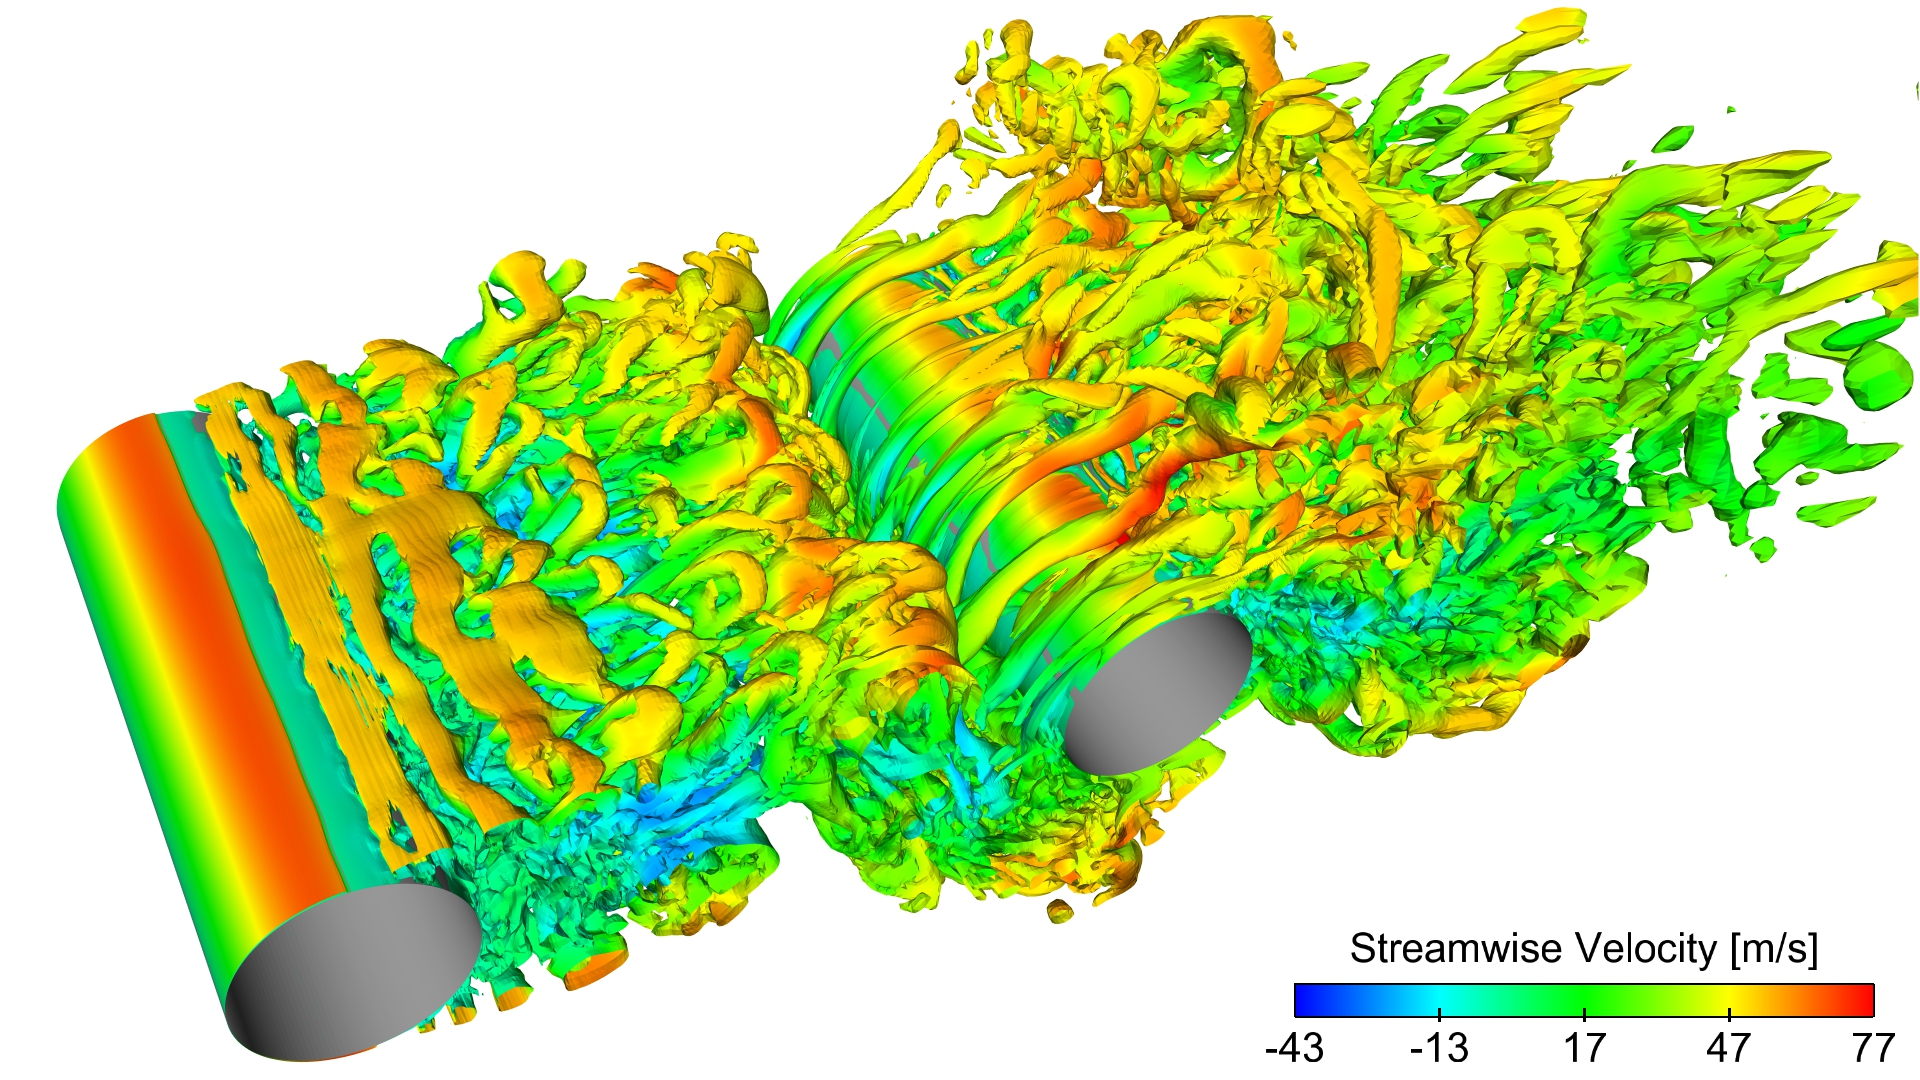
\includegraphics[width=0.45\textwidth]{ITC_Q_Criteria}
  \caption{Q判据等值面图}
  \label{fig:ITC_Q_Criteria}
\end{figure}
\end{verbatim}
\begin{figure}[!htbp]
  \centering
  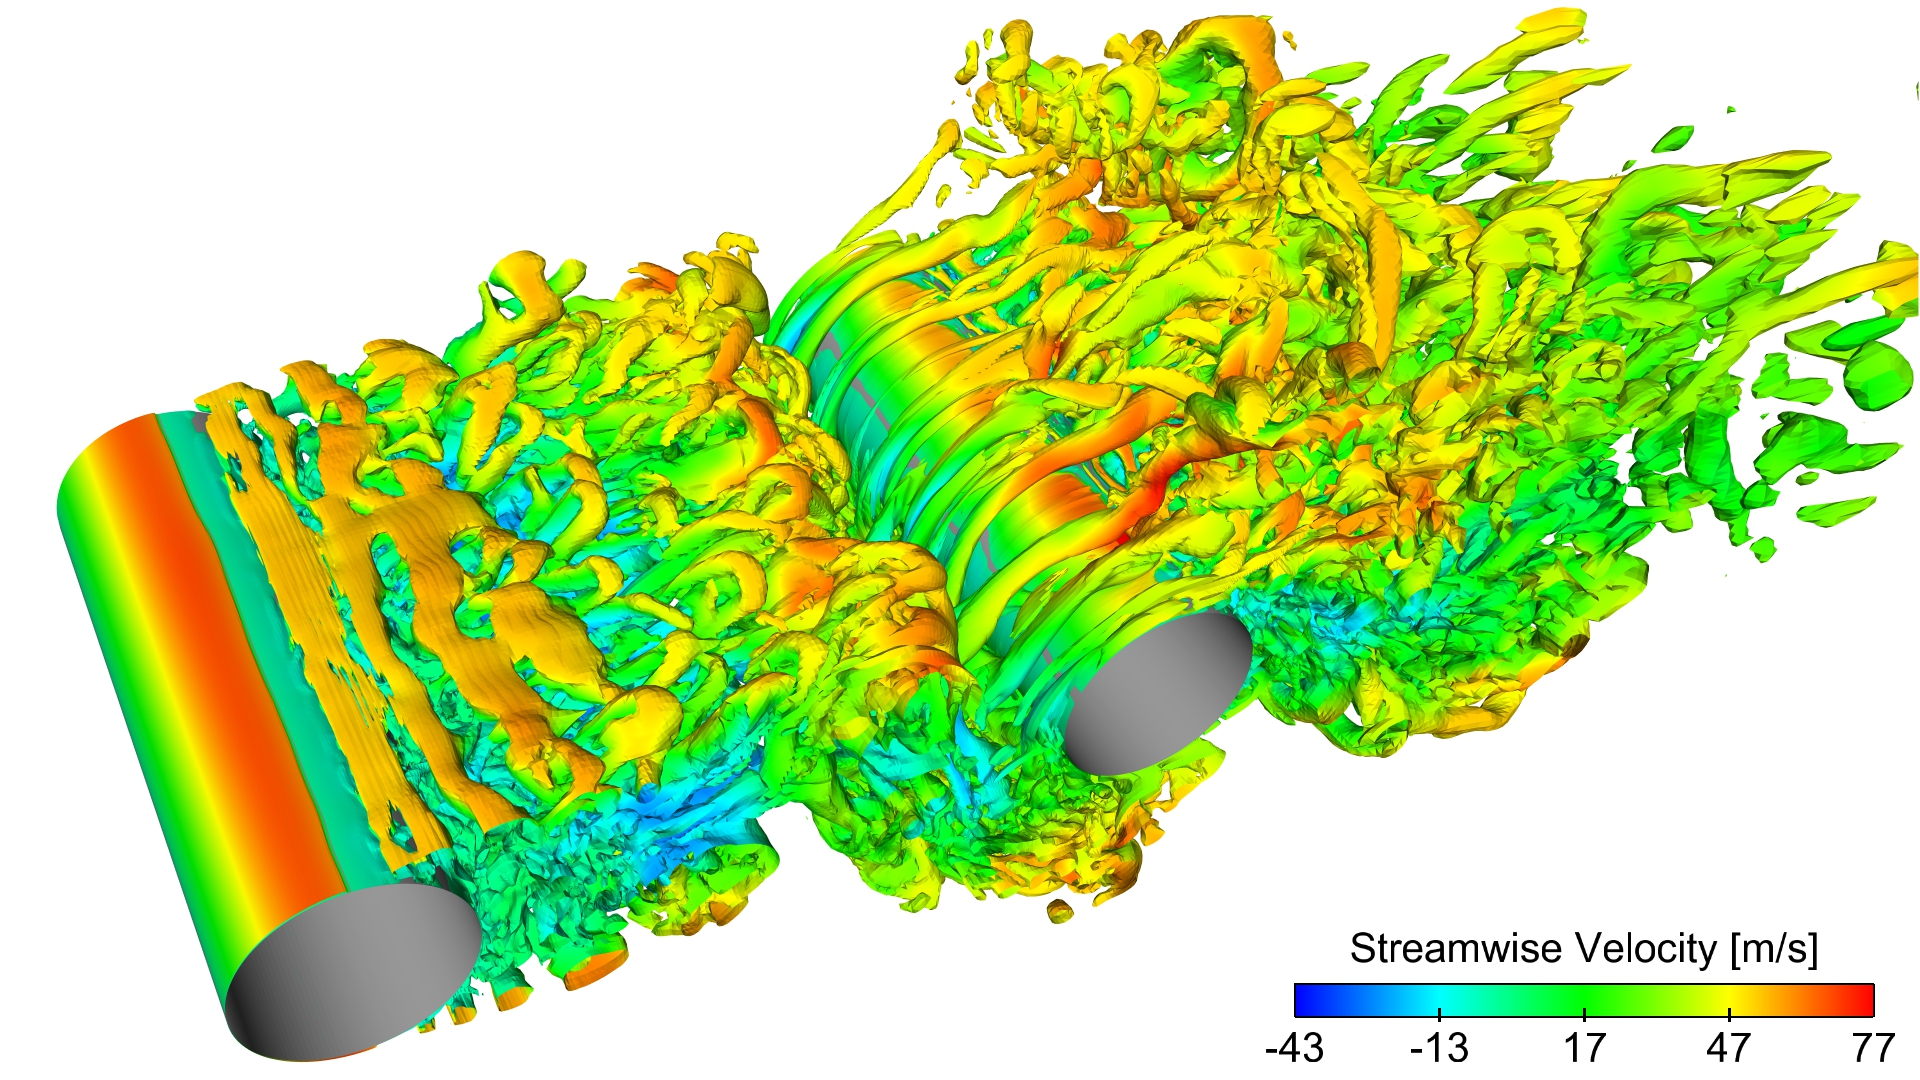
\includegraphics[width=0.45\textwidth]{ITC_Q_Criteria}
  \caption{Q判据等值面图}
  \label{fig:ITC_Q_Criteria}
\end{figure}

如果插图的空白区域过大,希望减少插入图片后的留白,以图片Y为例(图\ref{fig:Y}),可以使用如下代码模板:
\begin{verbatim}
\begin{figure}[!htbp]
  \centering
  %trim option's parameter order: left bottom right top
  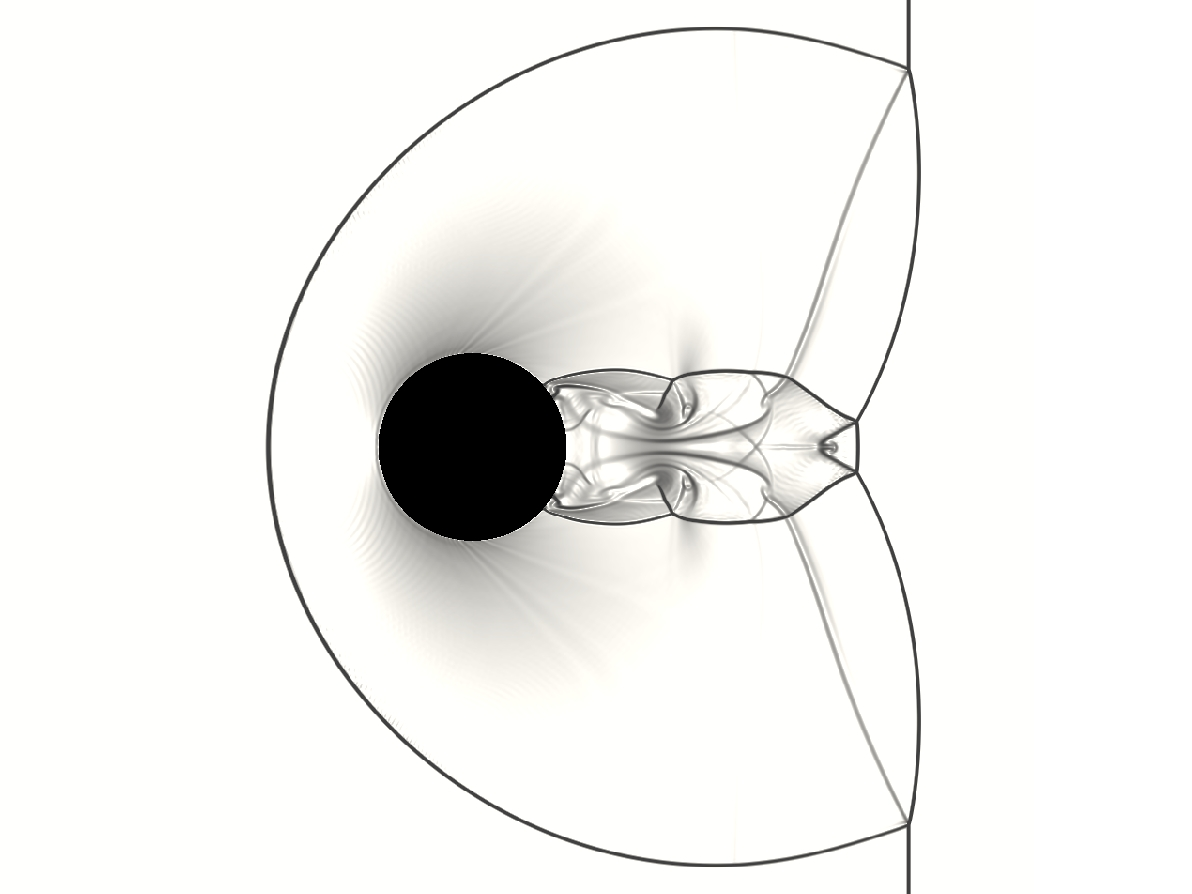
\includegraphics[trim = 30mm 0mm 30mm 0mm, clip, width=0.45\textwidth]{Y}
  \caption{Shock diffraction}
  \label{fig:Y}
\end{figure}
\end{verbatim}
\begin{figure}[!htbp]
  \centering
  %trim option's parameter order: left bottom right top
  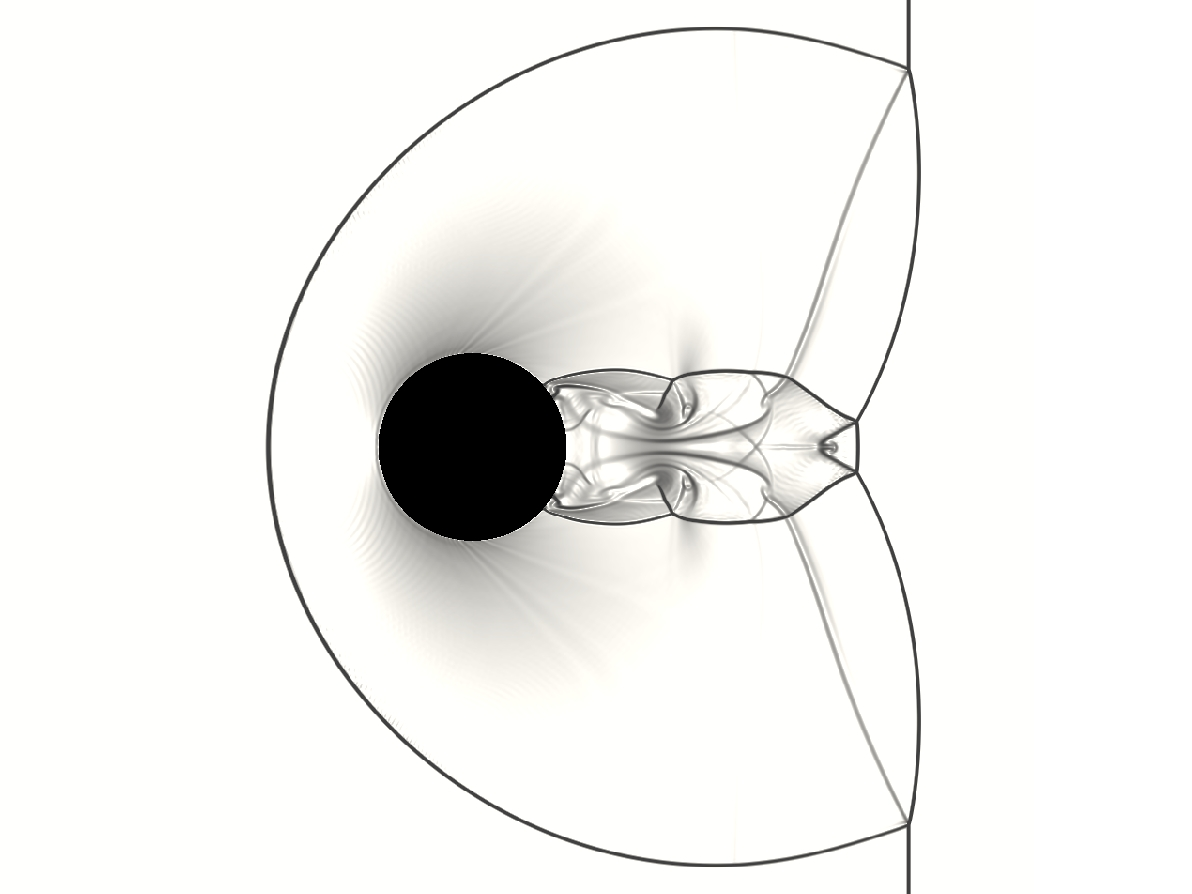
\includegraphics[trim = 30mm 0mm 30mm 0mm, clip, width=0.45\textwidth]{Y}
  \caption{Shock diffraction.}
  \label{fig:Y}
\end{figure}

多图的插入如图\ref{fig:HC_OASPL},其代码如下。
\begin{verbatim}
\begin{figure}[!htbp]
  \centering
  \begin{subfigure}[b]{0.45\textwidth}
    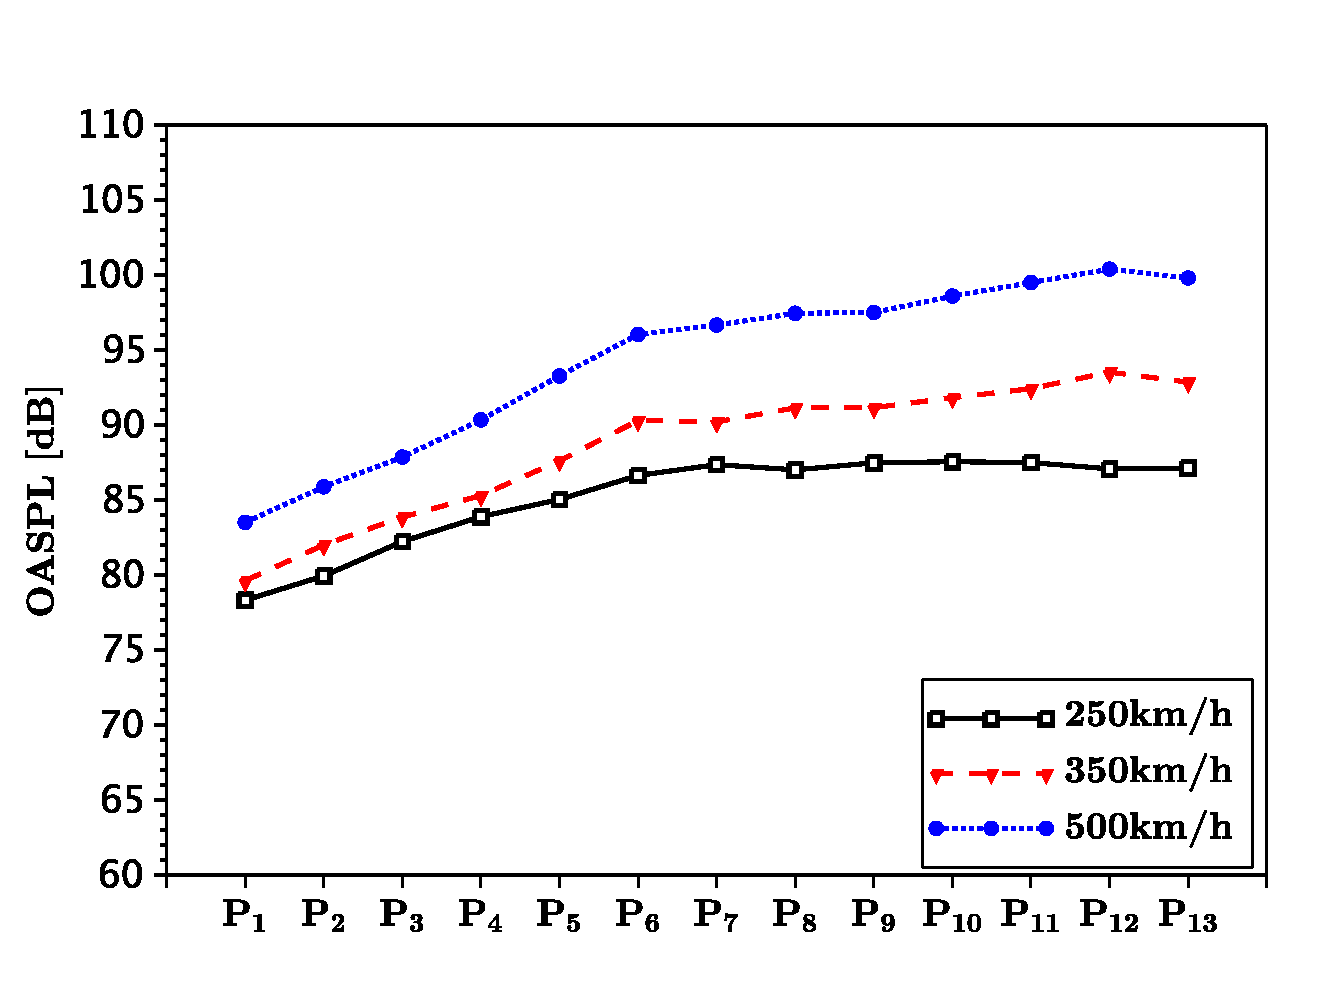
\includegraphics[width=\textwidth]{HC_OASPL_A}
    \caption{}
    \label{fig:HC_OASPL_A}
  \end{subfigure}%
  ~%add desired spacing
  \begin{subfigure}[b]{0.45\textwidth}
    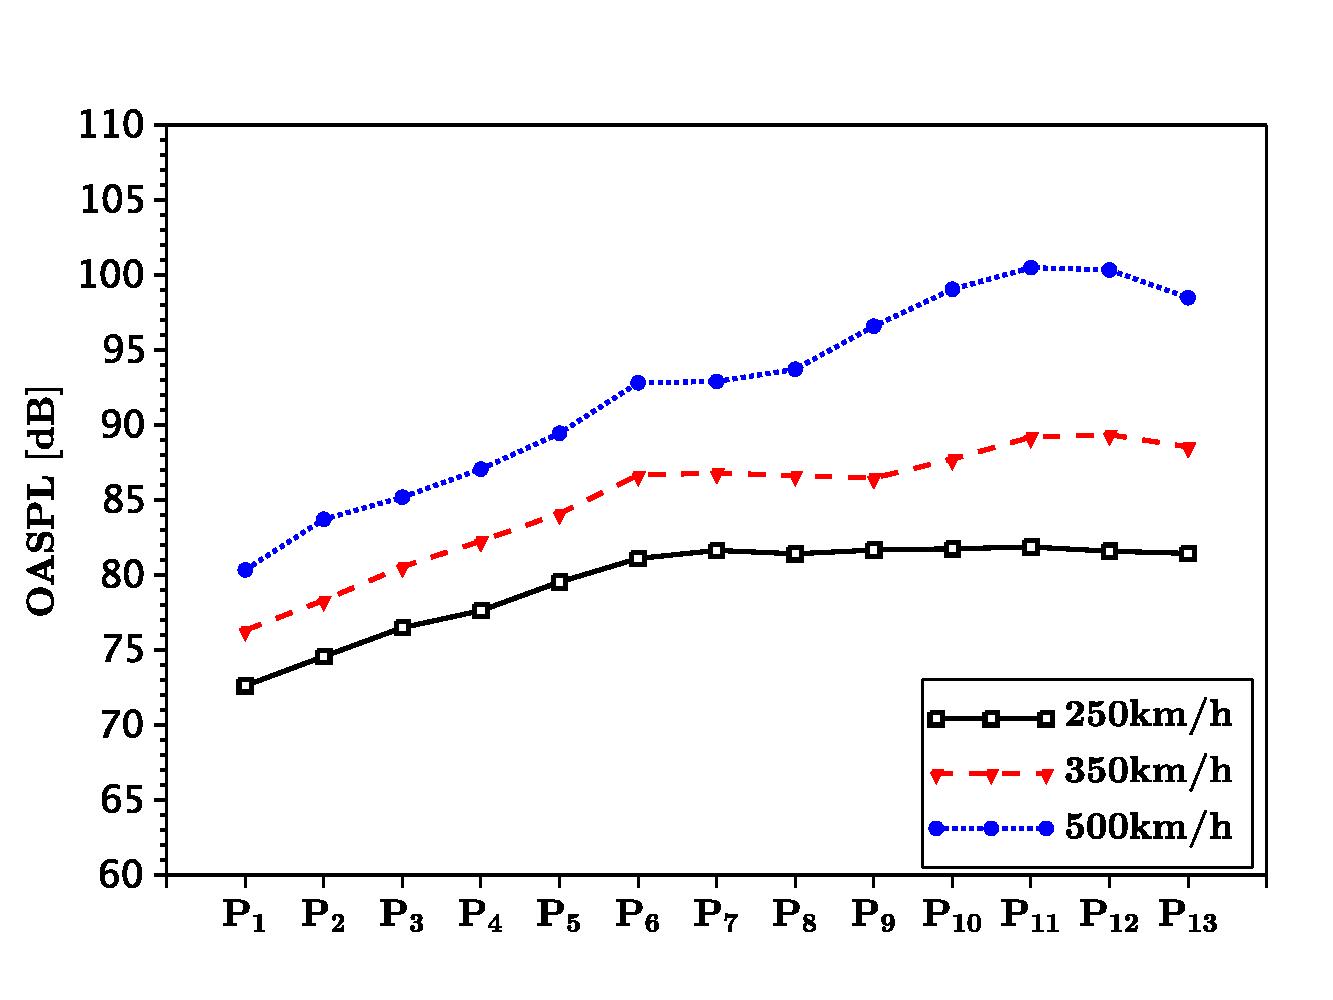
\includegraphics[width=\textwidth]{HC_OASPL_B}
    \caption{}
    \label{fig:HC_OASPL_B}
  \end{subfigure}
  \begin{subfigure}[b]{0.45\textwidth}
    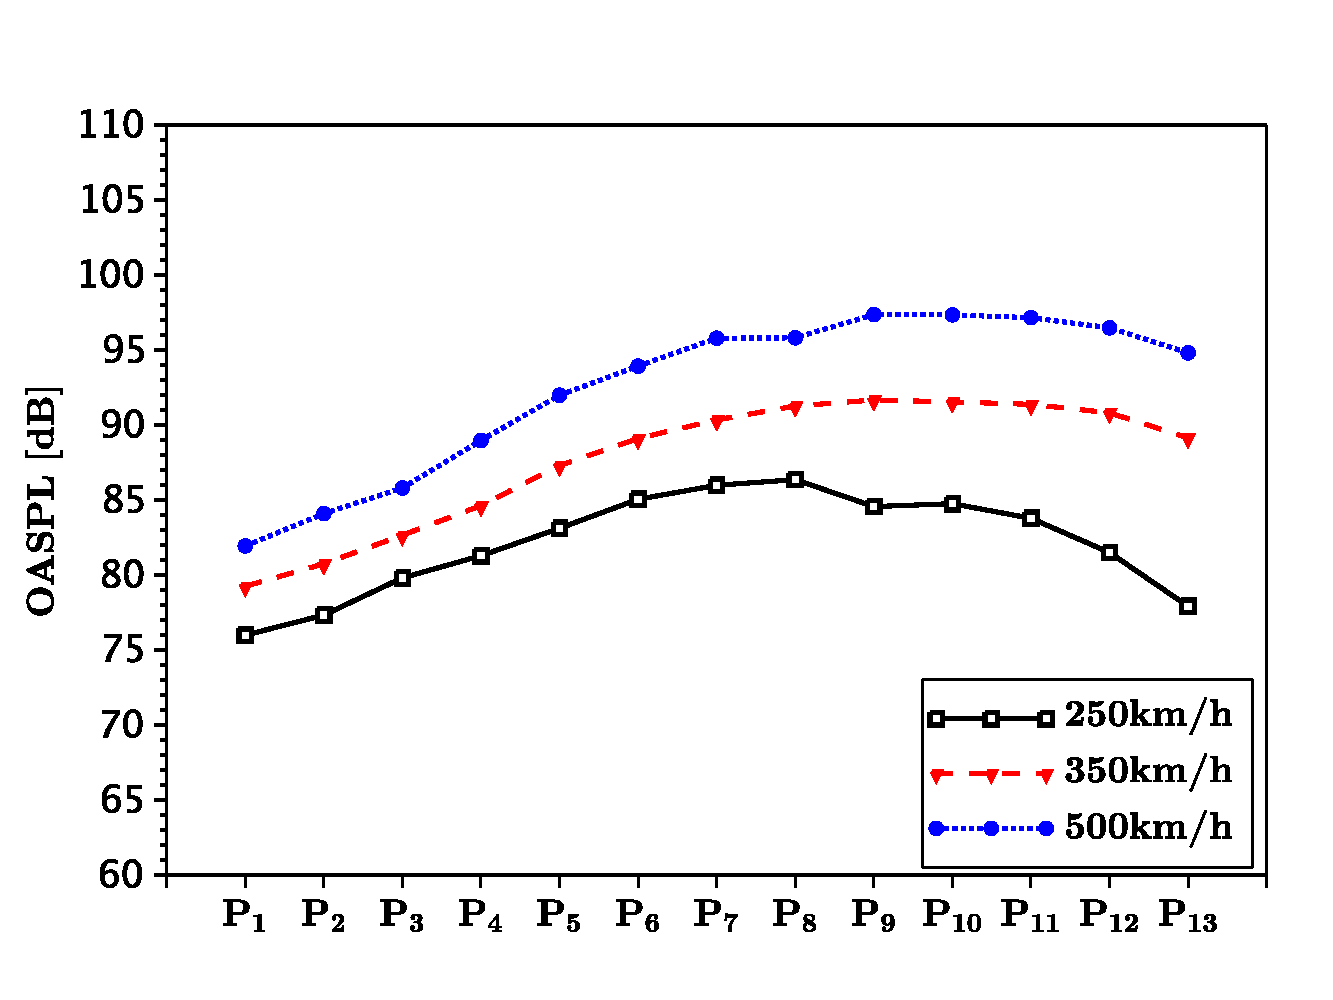
\includegraphics[width=\textwidth]{HC_OASPL_C}
    \caption{}
    \label{fig:HC_OASPL_C}
  \end{subfigure}%
  ~%add desired spacing
  \begin{subfigure}[b]{0.45\textwidth}
    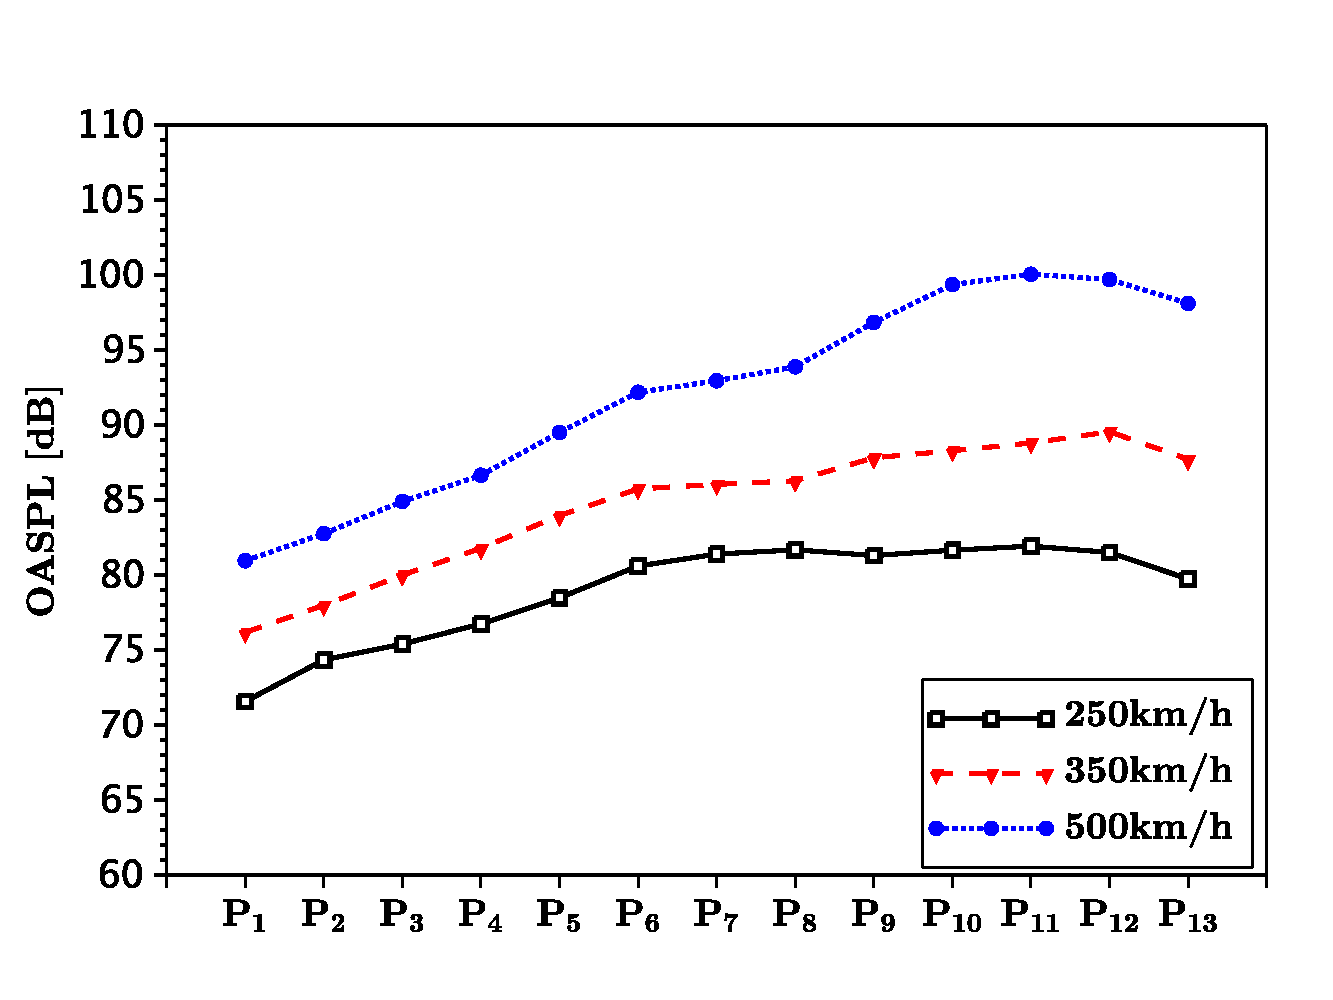
\includegraphics[width=\textwidth]{HC_OASPL_D}
    \caption{}
    \label{fig:HC_OASPL_D}
  \end{subfigure}
  \caption{总声压级。(a)$A$,(b)$B$,(c)$C$,(d)$D$}
  \label{fig:HC_OASPL}
\end{figure}
\end{verbatim}
\begin{figure}[!htbp]
  \centering
  \begin{subfigure}[b]{0.45\textwidth}
    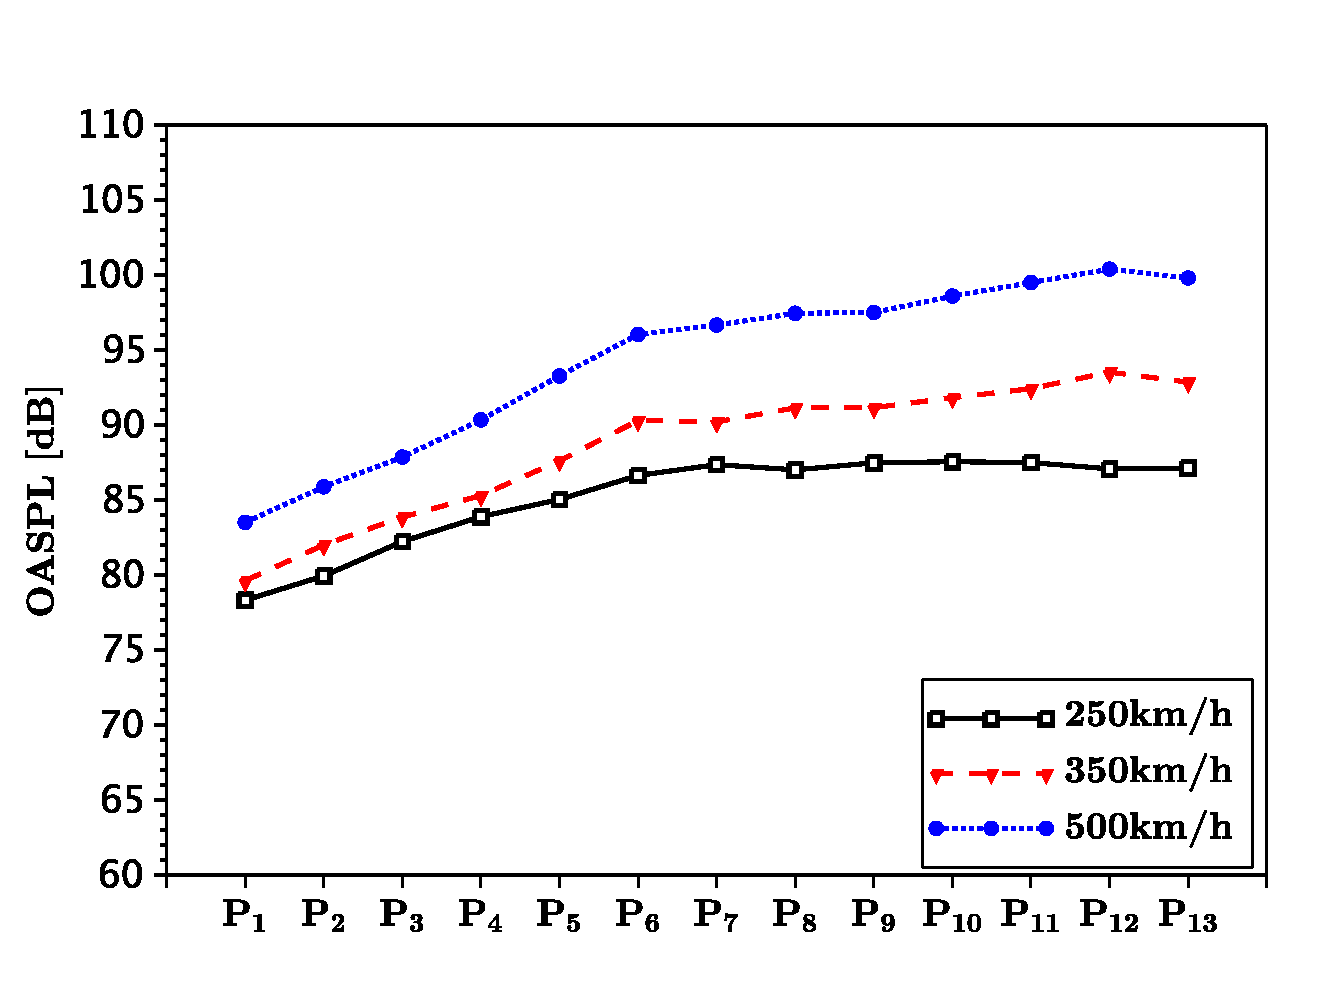
\includegraphics[width=\textwidth]{HC_OASPL_A}
    \caption{}
    \label{fig:HC_OASPL_A}
  \end{subfigure}%
  ~%add desired spacing
  \begin{subfigure}[b]{0.45\textwidth}
    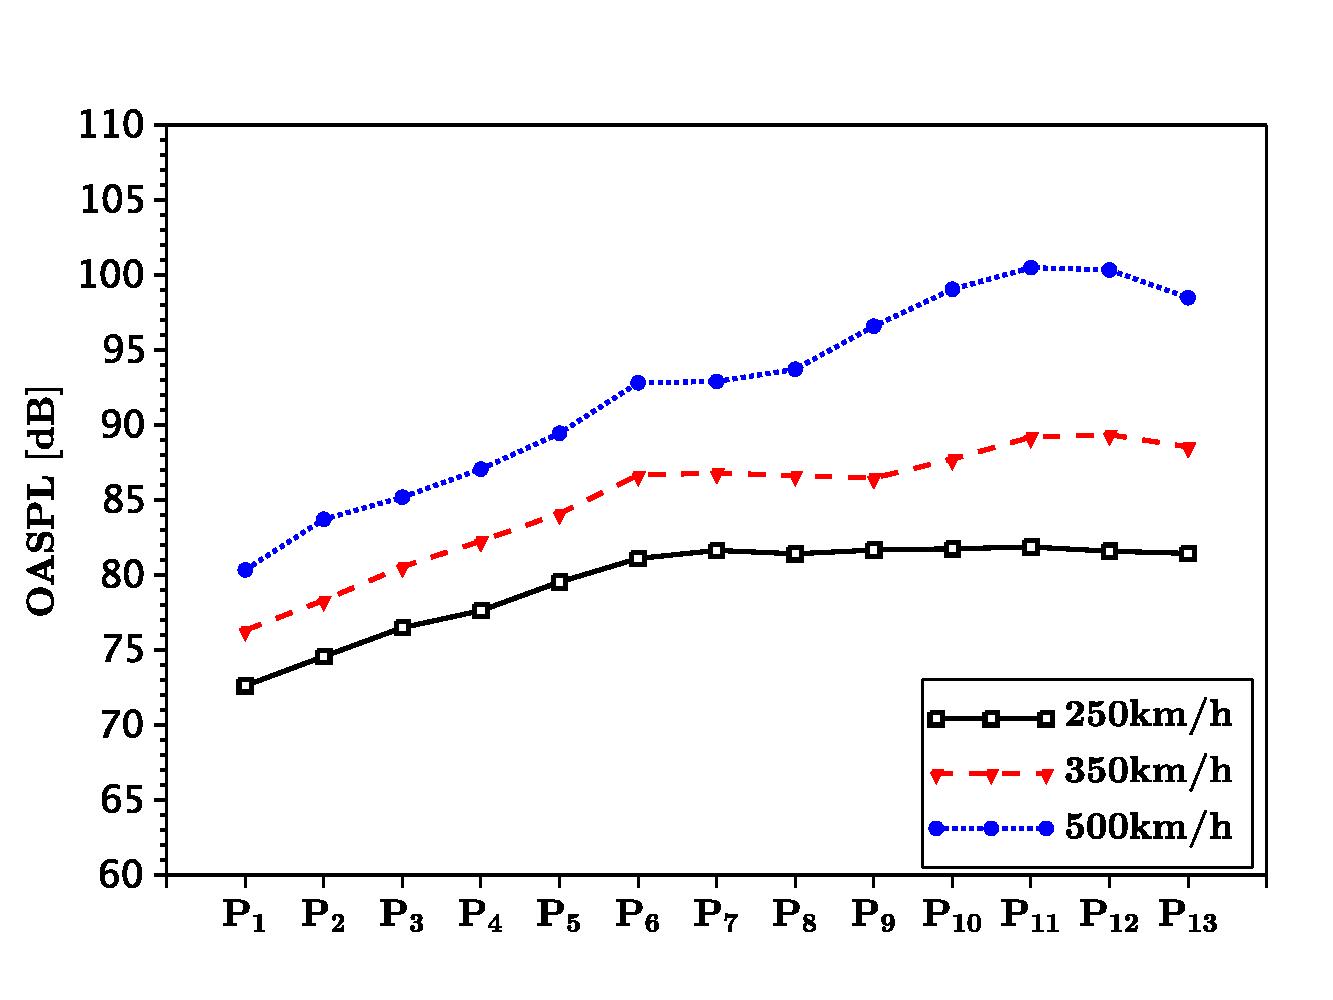
\includegraphics[width=\textwidth]{HC_OASPL_B}
    \caption{}
    \label{fig:HC_OASPL_B}
  \end{subfigure}
  \begin{subfigure}[b]{0.45\textwidth}
    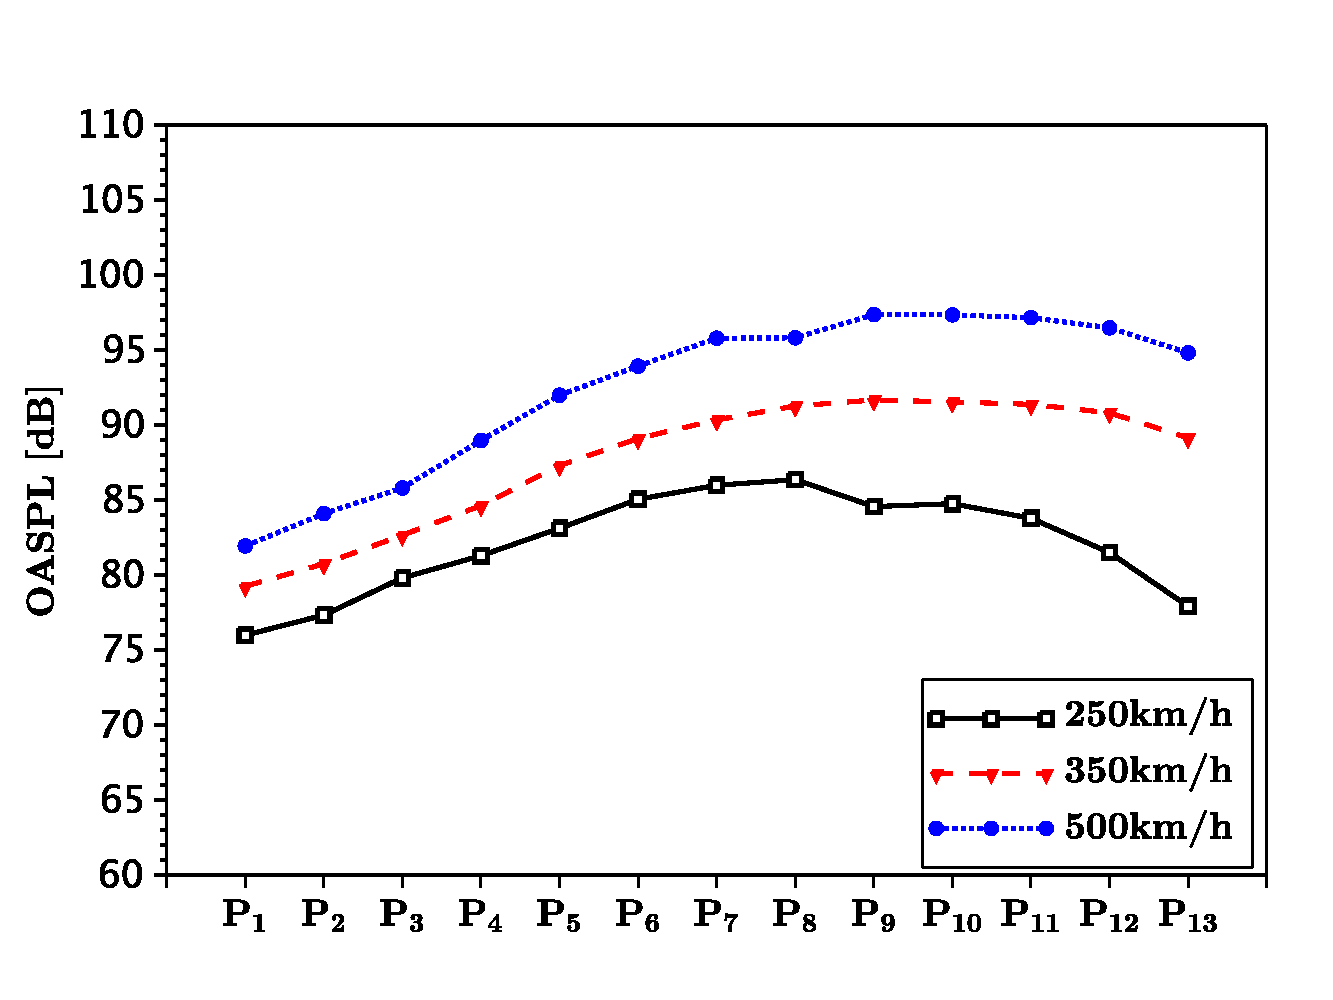
\includegraphics[width=\textwidth]{HC_OASPL_C}
    \caption{}
    \label{fig:HC_OASPL_C}
  \end{subfigure}%
  ~%add desired spacing
  \begin{subfigure}[b]{0.45\textwidth}
    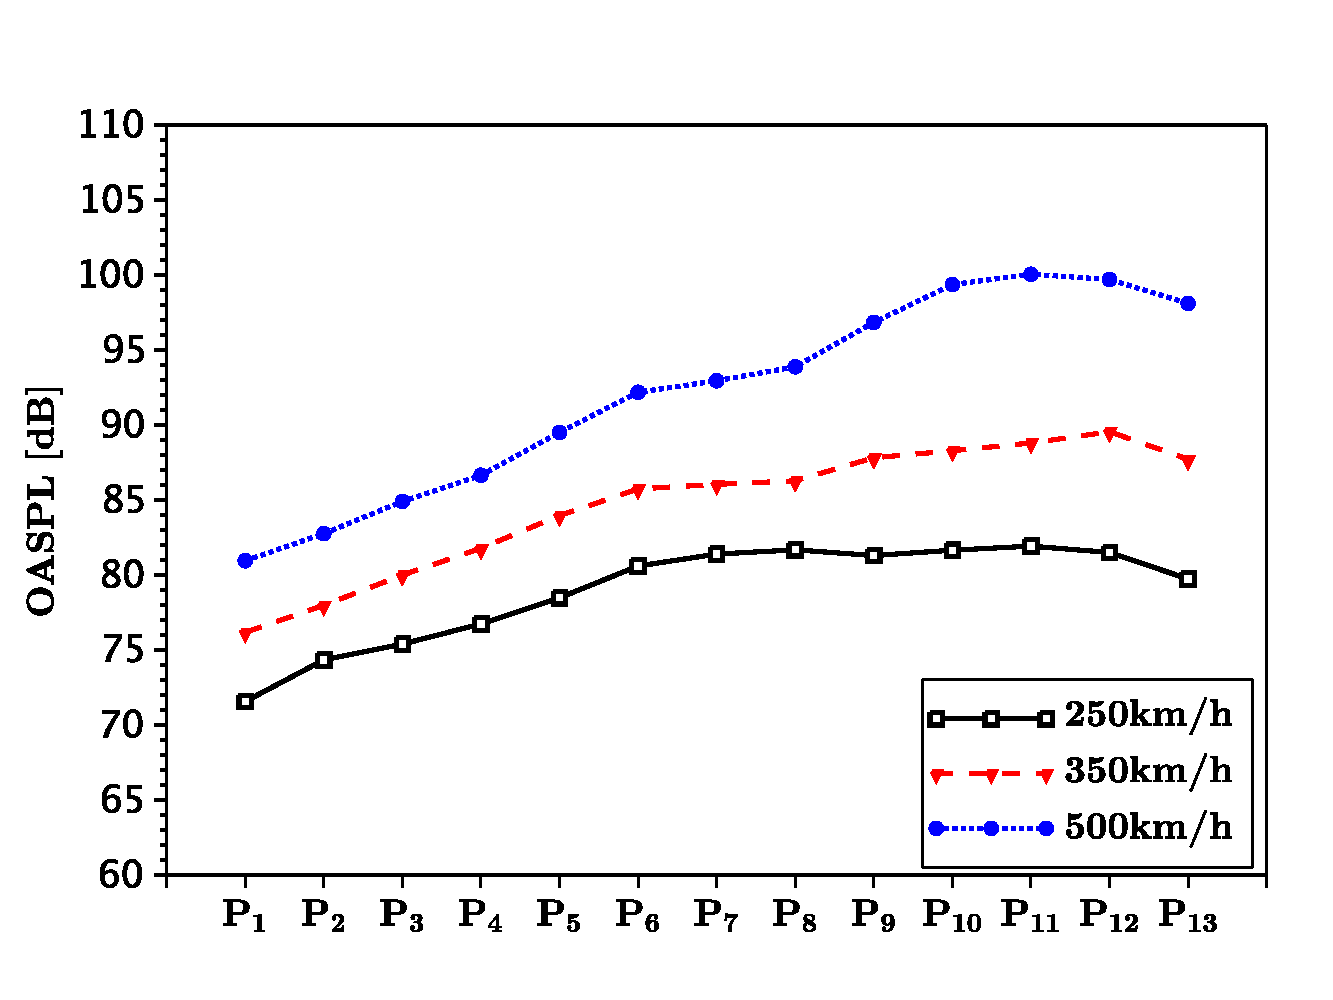
\includegraphics[width=\textwidth]{HC_OASPL_D}
    \caption{}
    \label{fig:HC_OASPL_D}
  \end{subfigure}
  \caption{总声压级。(a)$A$,(b)$B$,(c)$C$,(d)$D$}
  \label{fig:HC_OASPL}
\end{figure}

撰写论文中,插图和制表常用到的命令,已在\textbf{Useful Commands.txt}这个文本中给出了参考代码,大家只需copy使用即可。

\subsection{参考文献引用}

参考文献引用过程以实例进行介绍,假设需要引用名为Document Preparation System的文献,步骤如下:

1)使用google scholar搜索Document Preparation System,在目标条目下点击Cite,展开后选择Import into BibTeX打开此文章的BibTeX索引信息,将它们copy添加到ref.bib文件中(此文件位于Biblio文件夹下)。

2)你会发现索引信息中第一行为 \verb|@article{lamport1986document,|。其中 \verb|lamport1986document| 即为此文献的label (\textbf{中文文献也必须使用英文label},一般遵照:姓氏拼音+年份+标题第一字拼音的格式),想要在论文中索引此文献,有两种索引模式:

textual:\verb|\citet{lamport1986document}|。正如此处所示 \citet{lamport1986document}; 

parenthetical:\verb|\citep{lamport1986document}|。正如此处所示 \citep{lamport1986document}。

\textbf{多文献索引用英文逗号隔开}:

\verb|\citep{lamport1986document,chen2005zhulu}|。正如此处所示 \citep{lamport1986document,chen2005zhulu}

如此,即完成了文献的索引,请查看下本文档的参考文献一章,看看是不是就是这么简单呢?是的,就是这么简单!

不同文献样式和引用样式可在Thesis.tex中对commons.sty设置实现,如:

\verb+\usepackage[numbered]{commons}+ $\%$ default citation style. textual: Jones [1]; parenthetical: [1]

\verb+\usepackage[authoryear]{commons}+ $\%$ author year citation style. textual: Jones (1995); parenthetical: (Jones, 1995)

\verb+\usepackage[alpha]{commons}+ $\%$ alpha citation style. textual: not available; parenthetical: [Jon95]

若需将所有的上标改为嵌入式标注,则可在commons.sty 174行附近使用

\verb|\RequirePackage[square,comma,numbers,sort&compress]{natbib}|

的设置替换

\verb|\RequirePackage[square,comma,super,sort&compress]{natbib}|

如只希望在某些特定情形将上标改为嵌入式标注,则可使用

textural:\verb|\citepns{lamport1986document,chen2005zhulu}|。正如此处所示\citepns{lamport1986document,chen2005zhulu}

parenthetical:\verb|\citetns{lamport1986document,chen2005zhulu}|。正如此处所示\citetns{lamport1986document,chen2005zhulu}

参考文献索引更为详细的信息,请见Wikibook\citep{wikibook2014latex}。

\section{常见使用问题}

\begin{enumerate}
  \item 模板文档的编码为UTF-8编码。所有文件都必须采用UTF-8编码,否则编译后生成的文档将出现乱码文本。若出现文本编辑器无法打开文档或打开文档乱码的问题,请检查您使用的编辑器对UTF-8编码的支持,如果使用WinEdt作为文本编辑器,应在其

  options --》 Preferences --》 wrapping

  选项卡下将两种 Wrapping Modes 中的内容:

  TeX;HTML;ANSI;ASCII|DTX...

  修改为:

  TeX;\textbf{UTF-8|ACP;}HTML;ANSI;ASCII|DTX...

  同时,取消

  options --》 Preferences --》 Unicode

  中的Enable ANSI Format...选项。
  \item 推荐选择xelatex编译引擎编译。Compile.bat的默认设定为xelatex编译引擎。你也可以选择不使用此脚本编译,如直接使用 \TeX{}文本编辑器编译。注:\TeX{}文本编辑器编译的默认设定为pdflatex编译引擎,若选择xelatex编译引擎,请进入下拉菜单进行选择。为正确生成引用链接,编译步骤为: xelatex + bibtex + xelatex + xelatex。
  \item Texmaker使用简介
      \begin{enumerate}
          \item 使用 Texmaker 打开文档 Thesis.tex。
          \item 菜单 Options -> Define Current Document As 'Master Document'
          \item 菜单 User -> User Commands -> Edit User Commands -> Input Menu Item as 'Auto Build' -> Click 'wizard' -> add: xelatex + bibtex + xelatex + xelatex + pdf viewer -> Click 'OK'
          \item 使用 Auto Build 编译带有未生成引用链接的源文件,可以仅使用 xelatex 编译带有已经正确生成引用链接的源文件。
          \item 编译完成,View PDF,在pdf中'ctrl+click'可链接到相对应的源文件。
      \end{enumerate}
  \item 若编译过程中出现无法找到某些package的错误,如无法找到xcolor.sty,mathtools.sty,ctexbook.sty,newtext.sty等,\TeX{}编译程序一般可以自动下载和安装相应的文件,否则,请进入\LaTeX{}软件的Package Manager (Admin)确认启用Repository--Synchronize状态。下次编译过程中\TeX{}编译程序一般将自动下载安装\LaTeX{}宏包库。
  \item 模版在设计之初就尽可能地考虑了适应性。致谢,简历及攻读学位期间发表的学术论文与科研成果等几乎所有条目都是通过最为通用的
       
       \verb+\chapter{item name}+  and \verb+\section*{item name}+

       来显式实现的 (请仔细观察下Frontpage.tex, Prematter.tex, Backmatter.tex),从而你可以随意添加,放置,和修改他们,如同一般章节。对于图表目录名称则可在ucasthesis.cfg中进行修改。
   \item 设置正文行距: 在 custom.sty 99行附近, 修改

       \verb|\linespread{1.3}|

       设置参考文献行距: 在 custom.sty 103行附近, 修改/注掉

       \verb|\setlength{\bibsep}{0.0pt plus 0.3ex}|

       将subsection显示到目录当中: 在 custom.sty 107行附近, 将1改为2就可以了

       \verb|\setcounter{tocdepth}{1}% the depth for the Table of Contents.|

       如果需设置图2.3为图2-3,可将如下命令添加custom.sty中:

       \begin{verbatim}
\renewcommand{\theequation}{\arabic{chapter}-\arabic{equation}}
\renewcommand{\thefigure}{\arabic{chapter}-\arabic{figure}}
\renewcommand{\thetable}{\arabic{chapter}-\arabic{table}}
      \end{verbatim}
  \item 字体控制。如果对字体控制有较高需求,请选择xelatex编译引擎,并在commons.sty中设置需要的字体,如启用Times New Roman 作为英文字体,在commons.sty的105行附近设置:

      \verb+\setmainfont{Times New Roman}+
  \item 在某些情况下拷贝pdf文档内容到word时存在乱码。
      解决方式是选择安装adobe相应的字体库,请在公共网站(如百度云盘:\url{http://pan.baidu.com/share/home?uk=3188136325&view=share#category/type=0})搜索并下载如下四种中文字体文件:
      \begin{enumerate}
          \item AdobeFangsongStd-Regular.otf (adobe 仿宋)
          \item AdobeHeitiStd-Regular.otf(adobe 黑体)
          \item AdobeKaitiStd-Regular.otf(adobe 楷体)
          \item AdobeSongStd-Light.otf(adobe 宋体)
      \end{enumerate}
      下载字体文件后,双击安装相应字体。
      
      在Thesis.tex中设置启用adobe的字体:

      \verb+\documentclass[doublesided,fontset=adobe]{Style/ucasthesis}%+

      如果\LaTeX{}软件版本比较老旧,如Linux用户,ctex宏包没有更新,设置启用adobe的字体则为:

      \verb+\documentclass[doublesided,adobefonts]{Style/ucasthesis}%+
     
     最后选择xelatex编译引擎编译。

     因为模版的设定考虑兼顾不同操作系统(Windows, Linux, Mac OS)并兼顾pdflatex和xelatex,为了模版的健壮性,上述方案并未作为原始设定。
 \item 页眉页脚的设定在commons.sty的底部。始于323行附近的frontmatterstyle,mainmatterstyle,和backmatterstyle分别用于定义前言,主要内容,和附录的页眉页脚样式。一般默认情况下每一章的第一页不应显示页眉页脚,若想修改此行为,请将377-379行附近的plain样式定义注空即可。即修改为

\begin{verbatim}
\fancypagestyle{plain}{%
    %\fancyhf{}% clear fields
    %\renewcommand{\headrulewidth}{0pt}% header rule
    %\renewcommand{\footrulewidth}{0pt}% footer rule
}
\end{verbatim}
     
     关于页眉页脚各个命令的作用和意义请参见fancyhdr的用户文档 \url{https://www.ctan.org/pkg/fancyhdr?lang=en}。如果需要在页眉页脚中添加章节字样,请使用
      \begin{enumerate}
          \item \verb+\CTEXthechapter+  显示: 第X章
          \item \verb+\CTEXthesection+  显示: 第X节
      \end{enumerate}
      参见ctex宏包用户文档 \url{http://ctan.mirror.rafal.ca/language/chinese/ctex/ctex.pdf}
  \item 一般规范下,每一章应开始于奇数页。从而若前一章结束于奇数页,则一空白页将被插入以保证上述规则。如果想修改规则以取消空白页,有如下三种方案:
\begin{itemize}
    \item 在thesis.tex的documentclass中使用singlesided替代doublesided选项。这一命令使文档不区分奇偶页,因此章可以开始于任意页。此方案将移除所有的空白页,包括封面处的。同时,页面页脚的设定不再区分奇偶页。
    \item 可以在ucasthesis.cls文件中106行附近,将cleardoublepage命令的定义修改为:

      \verb|\def\cleardoublepage{\clearpage}|

      这一命令使产生空白页的机制失效。这一方案将移除所有的空白页,包括封面处的。但与方案一不同的是,页面页脚的设定可以区分奇偶页。
  \item 在thesis.tex的documentclass中添加openany选项(openany与doublesided和printcopy都可搭配)。这一命令使章可以开始于任意页。同时,将custom.sty中86行和thesis.tex中88行附近的cleardoublepage改为clearpage。此方案将移除所有的用于调整章的起始位置的空白页,而不包括封面处的。同时,页面页脚的设定可以区分奇偶页。
\end{itemize}
      无论哪种方案都需要注意对页眉页脚的影响并做出合适的调整。个人的推荐是采用默认设置,尽量避免将精力花在这些无关紧要的细节上。\LaTeX{}的特点是标准化,而其导致的问题则是任何脱离标准的修改都将花费相当的精力。对于电子档的论文,在thesis.tex的documentclass中,若不想使用doublesided,则可使用singlesided来减少空白页。而对于打印版,启用printcopy选项以替换doublesided/singlesided选项,这样可使奇偶页的排版在打印装订后更美观。
  \item 若pdflatex编译出现pdfTeX error (font expansion): auto expansion is only possible with scalable fonts。是因为MikTex安装后字体配置异常,请进入软件的package manager更新你的\LaTeX{}宏包库,并请进入
      
      \verb+C:\Program Files\MiKTeX 2.9\miktex\bin\x64+

       找到并运行updmap.exe。
    \item 部分同学留意到一个所谓的新的模板要求,那个模板是一位学生发布的,而其英文封面的设定不满足中国科学院大学学位论文封面设定。因中国科学院大学学位论文撰写规定只是限定了封面格式但是没有要求具体的内容格式,部分所因为图方便省事就直接将其作为了模板发布到了所内。但是,迄今为止学校官网上的撰写规定和模板(\url{http://onestop.ucas.edu.cn/home/info/abc167cb-4589-4e05-b014-052fa9291d0c/1})未做出任何修改,亦未发表任何官方声明表示模板需要修改。所以,当前模板将不会在官方版发布之前做出调整。
\end{enumerate}

\nocite{*}% show all the bibliography entries
